% \documentclass{report}

% \usepackage{subcaption} % package for subfigures
% \usepackage{hyperref}  % package for linking figures etc
% \usepackage{enumitem}  % package for description with bullets
% \usepackage{graphicx}  % package for importing images
% \usepackage{mathtools} % package for math equation
% \usepackage{mathrsfs}  % package for math font
% \usepackage{indentfirst} % package for getting ident after section or paragraph
% \usepackage[export]{adjustbox}
% \usepackage{longtable} % package for multi pages tables
% \usepackage{multirow}  % package for tables, multirow
% % \usepackage{amsmath}

% \setlength{\parindent}{2em} % how much indent to use when we start a paragraph

% \graphicspath{ {./theory/figures/} }       % path for images

% \begin{document}

\chapter{Classification stage}
\section{Description}
After getting all proposed tubes, it's time to do classification. As classifiers we use several approaches includingn
a Recursive Neural Network (RNN) Classifier, a Support Vector Machine (SVM) Classifier and a Multilayer perceptron (MLP).

\begin{figure}[h]
  % 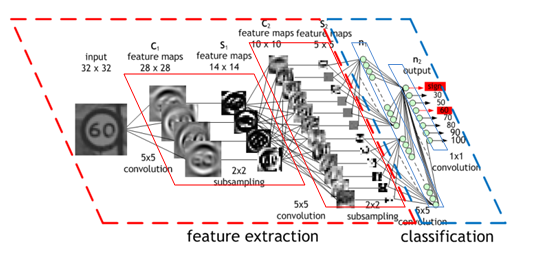
\includegraphics[scale=0.7]{convolutional_neural_network_structure} \]
  \centering
  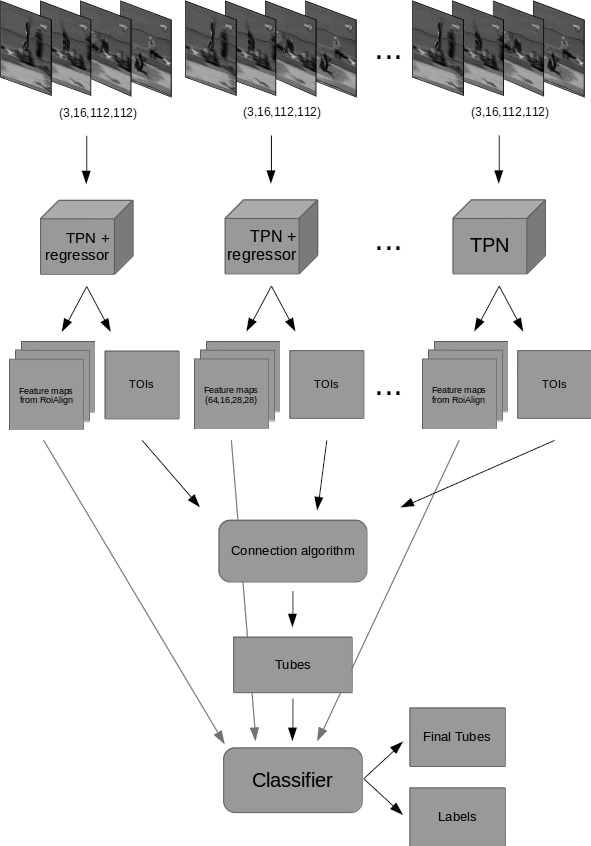
\includegraphics[scale=0.42]{model_prenms}
  \caption{Structure of the whole network}
  \label{fig:whole_network}
\end{figure}

The whole procedure of classification is consisted from the following steps:
\begin{enumerate}
\item Seperate video into small video clips. Feed TPN network those video clips and get as output
  k-proposed ToIs and their corresponding features for each video clip.
\item Connect the proposed ToIs in order to get video tubes which may contain an action.
\item For each candidate video tube, which is a sequence of ToIs, feed it into the classifier
  for verification.
\end{enumerate}

The general structure of the whole network is depicted in figure \ref{fig:whole_network}, in which we can see the previous steps if we
follow the arrows.  \par
In first steps of classification stage we refer only to JHMDB dataset because it has smaller number of video than UCF dataset which
helped us save a lot of time and resources. That's because  we performed most experiments only JHMDB and after we found the optimal
situation, we implemented to UCF-dataset, too. 

\section{Preparing data for classification -  RNN Classifier}

% \textbf{(Pending... Introduction about Linear and RNN classifiers)}
\textbf{(Pending.. also an image of RNN classifier)}
Recurrent neural networks, or RNNs for short, are a type of neural network that was designed to learn from sequence data,
such as sequences of observations over time, or a sequence of words in a sentence.
RNN takes many input vectors to process them and output other vectors.
It can be roughly pictured like in the Figure \ref{fig:rnn} below,
imagining each rectangle has a vectorial depth and other special hidden quirks in the image below.
For our case, we choose \textbf{many to one} approach, because we want only one prediction, at the end of
the action tube. \par
\begin{figure}[h]
  \centering
  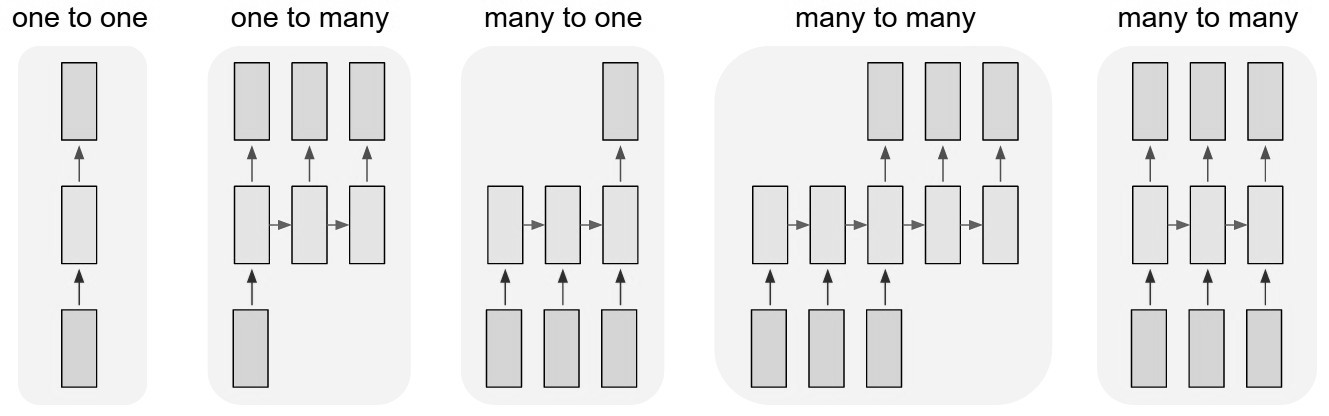
\includegraphics[width=1.\textwidth]{rnn.jpeg}
  \caption{Types of RNN}
  \label{fig:rnn}
\end{figure}



In order to train our classifier, we have to execute the previous steps for each video. However, each video
has different number of frames and reserves too much memory in the GPU. In order to deal with this situation,
we give as input one video per GPU. So we can handle 4 videos simultaneously. This means that a regular
training session takes too much time for just 1 epoch. \par
The solution we came with, is to precompute the features for both positive video tubes and negative video tubes.
Then we feed those features to our classifier and we train it in order to disciminate their classes.
At first, we extract only groundtruth video tubes' features and the double number of background video tubes. We chose this
ratio between positive and negative tubes inspired by \cite{jjfaster2rcnn}, in which it has 0.25 ratio between foreground
and background rois and chooses 128 roi in total. Respectively, we chose a little bigger ratio because we have only 1 groundtruth
video tube in each video. So, for each video we got 3 video tubes in total, 1 for positive and 2 for background. We considered
background tubes those whose overlap scores with groundtruth tubes are $ \ge 0.1 $ and $ \le 0.3 $. \par

Then, after extracting those features, we trained both Linear and RNN classifiers. The Linear classifier needs a fixed input size,
so we used a pooling function in the dimension of the videos. So, at first we had a feature map of 3,512,16 dimensions and then we
get as output a feature maps of 512,16 dimensions. We used both max and mean pooling as show in the results below. For the RNN
classifier, we do not use any pooling function before feeding it. For both classifiers, at first, we didn't considered a fixed
threshold for confidence score. 

\begin{table}[h]
  \centering
  \begin{tabular}{|| c || c  c  c ||}
    \hline
    \multirow{2}{*}{\textbf{Classifier}} & {} & \textbf{mAP} & {} \\
    {} & 0.5 & 0.4 & 0.3 \\
    \hline
    Linear & TODO & TODO & TODO \\
    \hline
    RNN    & 11.3 & 14.14 & 14.84 \\
    \hline
  \end{tabular}
  \caption{}
  \label{fig:rnn_linear}
\end{table}

  
\textbf{(Pending results RNN... Table)}
\textbf{(Pending results RNN... commentary)}
% The results are disappointing.
% As we can see in the table, RNN classifier cannot classify very well because, probably, the duration of the videos are so small
% so we stopped using it in jHMDB dataset. In the Linear classifier, we noticed that every tube is considered as background tube.
% That means that Linear classifier gets overfitted with trained data and cannot handle unknown data. So, we thought that we
% need a classifier which can \"learn\" very easily, with little data. So we chose to try a support vector machine classifier.

\section{Support Vector Machine (SVM)}
\subsection{First steps}
SVMs are classifiers defined by a separating hyperplane between trained data in a N-dimensional space. The main advantage of using a SVM
is that can get very good classification results when we have few data available. 
\textbf{write more introduction and a pic, Pending...} \par
The use of SVM is inspired from \cite{Girshick:2015:FR:2919332.2920125} and it is trained using hard negative mining. 
This means that we have 1 classifier per class which has only 2 labels, positive and negative. We mark as positive the feature maps of the
groundtruth action, and as negative groundtruth actions from other classes, and feature maps from background classes.
As we know, SVM is driven by small number of examples near decision boundary. Our goal is to find a set of negatives that are the closest to
the seperating hyperplane. So in each iteration, we update this set of negatives adding those which our SVM didn't perform very well. Each
SVM is trained independently. \par
SVM code is take from Microsoft's Azure \href{https://github.com/Azure/ObjectDetectionUsingCntk} {github page} in which there is an implementation
of Fast RCNN using a SVM classifier. We didn't modify its parameters which means that it has a linear kernelr, uses  L2-norm as penalty and L1-norm
as loss during training. Also, we consider as hard-negatives the tubes that got score $ >  -1.0 $ during classification.\par
This whole process makes the choise of the negatives a crutial factor. In order to find the best policy,  we came with 5 different cases to consider
as negatives:
\begin{enumerate}
\item Negatives are other classes's positives and all the background tubes
\item Negatives are only all the background videos
\item Negatives are only other classes's positives
\item Negatives are other classes's positives and background tubes taken only from videos that contain a positive tube
\item Negatives are only background tubes taken from videos that contain a positive tube
\end{enumerate}

On top of that, we use 2 pooling functions in order to have a fixed input size. \par
In the next tables, we show our architecture's  mAP performance when we follow each one of the above policies. Also,
we experimented for 2 feature maps, \textit{(64,8,7,7)} and \textit{(256,8,7,7)} where 8 equals with the sample duration.
Both feature maps were extracted by using 3D RoiAlign procedure from feature maps with dimensions \textit{(64,8,28,28)} and
\textit{(256,8,7,7)} respectively (in the second case, we just add zeros in the feature map outsize from the bounding boxes for
each frame). Table \ref{table:svm_first_results} contains the first classification results. At first column we have the dimensions
of feature maps before pooling fuction, where k = 1,2,..5 . At second column we have feature maps' dimensions after pooling, and at
the next 2 column, the type of pooling function and the policy we followed. Finally in the last 3 collumns we have the mAP performance
when we have threshold equal with 0.3, 0.4 and 0.5 respectively. During validation, we keep only the best scoring tube because we know that
we have only 1 action per video.

\begin{center}
\begin{longtable}{||c | c | c| c||c c c||}

  \hline
  \multicolumn{2}{||c|}{\textbf{Dimensions}} & \multirow{2}{*}{ \textbf{Pooling}} &\multirow{2}{*}{\textbf{Type}} & \multicolumn{3}{|c||}{\textbf{mAP precision}}\\

   before & after &  {} & {} &  0.5 &  0.4 & 0.3 \\
 \hline   \hline
 \multirow{5}{*}{(k,64,8,7,7)} & \multirow{5}{*}{(1,64,8,7,7)} & \multirow{5}{*}{mean}  & 1 &  3.16 & 4.2 & 4.4    \\
  \cline{4-7}
  {} & {} & {} & 2 & 2.29 & 2.68 & 2.86    \\
    \cline{4-7}
  {} & {} & {} & 3 & 1.63 & 3.16 &  4  \\
    \cline{4-7}
  {} & {} & {} & 4 & 2.42 & 4.83 & 5.46  \\  
    \cline{4-7}
  {} & {} & {} & 5 & 0.89 &1.12 & 1.21  \\
  \hline
 \multirow{5}{*}{(k,64,8,7,7)} & \multirow{5}{*}{(1,64,8,7,7)} & \multirow{5}{*}{max}  & 1 & 1.11 & 2.35 & 2.71 \\
    \cline{4-7}
  {} & {} & {} & 2 & 2.31 & 2.62 & 2.64 \\
    \cline{4-7}
  {} & {} & {} & 3 & 1.11 & 2.35 & 2.71 \\
    \cline{4-7}
  {} & {} & {} & 4 & 1.41 & 2.76 & 3.84  \\
    \cline{4-7}
  {} & {} & {} & 5 & 0.33 & 0.51 &0.58  \\

  \hline   \hline

 \multirow{5}{*}{(k,256,8,7,7)} & \multirow{5}{*}{(1,256,8,7,7)} & \multirow{5}{*}{mean}  & 1 &  11.41 & 11.73 & 11.73 \\

    \cline{4-7}
  {} & {} & {} & 2 & 10.35 & 10.92 &11.89 \\
    \cline{4-7}
  {} & {} & {} & 3 & 8.93 & 9.64 & 9.94 \\
    \cline{4-7}
  {} & {} & {} & 4 & 12.1 & 13.04 &13.04 \\
    \cline{4-7}
  {} & {} & {} & 5 & 5.92 & 6.92 & 7.79 \\
    \hline
 \multirow{5}{*}{(k,256,8,7,7)} & \multirow{5}{*}{(1,256,8,7,7)} & \multirow{5}{*}{max}  & 1  & 22.07 & 24.4 & 25.77  \\
    \cline{4-7}
  {} & {} & {} & 2  & 14.07 & 16.56 & 17.74 \\
    \cline{4-7}
  {} & {} & {} & 3  & 14.22 & 18.94 &21.6 \\
    \cline{4-7}
  {} & {} & {} & 4  & 21.05 & 24.63 & 25.93 \\
    \cline{4-7}
  {} & {} & {} & 5  & 11.6 & 13.92 & 15.81 \\
  \hline   
  
  \caption{Our architecture's performance using 5 different policies and 2 different feature maps while pooling in
  tubes' dimension. With bold is the best scoring case}
  \label{table:svm_first_results}

\end{longtable} 
\end{center}

From the above results we notice that features map with dimension (256,8,7,7) outperform in all cases, both for mean and max pooling and
for all the policies. Also, we can see that max pooling outperforms mean pooling in all cases, too. Last but not least, we notice that policies
2, 3 and 5 give us the worst results which means that svm needs both data from other classes positives and from background tubes. 

\subsection{Modifying 3D Roi Align}
As we mentioned before, we extract from each tube its activation maps using 3D Roi Align procedure and we set equal to zero the pixels outside
of bounding boxes for each frame. We came with the idea that the enviroment surrounding the actor sometimes help us determine the class
of the action which is performed. This is base in the idea that 3D Convolutional Networks use the whole scene in order to classify the action
that is performed. We thought to extend a little each bounding box both in width and height. So, during Roi Align procedure, after resizing
the bounding box into the desired spatial scale  ( in our case 1/16 because original sample size = 112 and resized sample size = 7 )
we increase by 1 both width and height. According to that if we have a resized bounding box $( x_1,y_1,x_2,y_2) $ our new bounding box becomes
$ (max(0,x_1-0.5),max(0,y_1-0.5),min(7,x_2+0.5),min(7,y_2+0.5)) $ ( we use \textit{ min} and \textit{max} functions in order to avoid exceeding feature maps' limits).
We just experiment in policies 1 and 4 for both (256,8,7,7) and (64,8,7,7) feature maps as show in  Table \ref{table:svm_mod_roialign}


\begin{center}
\begin{longtable}{||c | c | c| c||c c c||}

  \hline
  \multicolumn{2}{||c|}{\textbf{Dimensions}} & \multirow{2}{*}{ \textbf{Pooling}} &\multirow{2}{*}{\textbf{Type}} & \multicolumn{3}{|c||}{\textbf{mAP precision}}\\

   before & after &  {} & {} &  0.3 &  0.4 & 0.5 \\
 \hline   \hline
 \multirow{2}{*}{(k,64,8,7,7)} & \multirow{2}{*}{(1,64,8,7,7)} & \multirow{2}{*}{mean}  & 1 & 9.75 & 11.92 & 13.34 \\
  \cline{4-7}
  {} & {} & {} & 4 &  5.74 &6.62 & 7.59 \\
  \hline
 \multirow{2}{*}{(k,64,8,7,7)} & \multirow{2}{*}{(1,64,8,7,7)} & \multirow{2}{*}{max}  & 1 &  6.46 & 10.26 & 10.83 \\
    \cline{4-7}
  {} & {} & {} & 4 & 4.19 & 6.27 & 7.52 \\
    \cline{4-7}
  \hline
  \caption{Our architecture's performance using 2 different policies and 2 different pooling methods using modified Roi Align.}
  \label{table:svm_mod_roialign}

\end{longtable} 
\end{center}


\textbf{Pending commetary...}
\\

\subsection{Temporal pooling}
After getting first results, we implement a temporal pooling function inspired from \cite{DBLP:journals/corr/HouCS17}. We need a
fixed input size for the SVM. However, our tubes' temporal stride varies from 2 to 5. So we use as fixed temporal pooling equal
with 2. As pooling function we use 3D max pooling, one for each filter of the feature map.  So for example, for an action tube
with 4 consecutive ToIs, we  have 4,256,8,7,7 as feature size. We seperate the feature map into 2 groups using \textit{linspace}
function and we reshape the feature map into 256,k,8,7,7 where k is the size of each group, After using 3D max pooling, we get
a feature map 256,8,7,7 so finally we concat them and get 2,256,8,7,7. In this case we didn't experiment with (64,8,7,7) feature
maps because it wouldn't performed better that (256,8,7,7) ferature maps as noticed from the previous section.

\begin{center}
\begin{longtable}{||c | c| c| c||c c c||}

  \hline
 \multicolumn{2}{||c|}{\textbf{Dimensions}} & \multirow{2}{*}{\textbf{Pooling}} &\multirow{2}{*}{ \textbf{Type}} &\multicolumn{3}{|c||}{\textbf{mAP precision}}\\

  before & after & {} & {} & 0.5 &  0.4 & 0.3\\
  \hline   \hline

  \multirow{4}{*}{k,256,8,7,7} & \multirow{4}{*}{2,256,8,7,7} & \multirow{2}{*}{RoiAlign}  & 1 & 25.07 & 26.91 & 29.11 \\
  \cline{4-7}
  {} & {} & {} & 4 &  23.27 & 25.96 & 28.25 \\
  \cline{3-7}
  {} & {} & \multirow{2}{*}{mod RoiAlign} & 1 & 7.01 & 9.69 & 10.52 \\
  \cline{4-7}
  {} & {} & {} & 4 & 5.5 & 7.25 & 8.99 \\
  \hline

  \caption{mAP results using temporal pooling for both RoiAlign approaches}
  \label{table:svm_temp_pooling}
\end{longtable} 
\end{center}

\subsection{Increasing sample duration to 16 frames}

\textbf{Pending description...}
\begin{center}
\begin{longtable}{||c | c| c| c||c c c||}

  \hline
 \multicolumn{2}{||c|}{\textbf{Dimensions}} & \multirow{2}{4.5em}{\textbf{Temporal Pooling}} &\multirow{2}{*}{ \textbf{Type}} &\multicolumn{3}{|c||}{\textbf{mAP precision}}\\

  before & after & {} & {} &  0.5 &  0.4 & 0.3 \\
  \hline   \hline

  \multirow{5}{*}{k,256,16,7,7} & \multirow{5}{*}{1,256,16,7,7} & \multirow{5}{*}{No}  & 1 & 23.4 & 27.57 &28.65  \\
  \cline{4-7}

  {} & {} & {} & 2 & Pending \\
  \cline{4-7}
  {} & {} & {} & 3 & Pending \\
  \cline{4-7}
  {} & {} & {} & 4 & 22.7 & 26.95 & 28.05 \\
  \cline{4-7}
  {} & {} & {} & 5 & Pending \\
  \hline

  \multirow{5}{*}{k,256,16,7,7} & \multirow{5}{*}{2,256,16,7,7} & \multirow{5}{*}{Yes}  & 1 & 21.12 & 24.07 & 24.36  \\
  \cline{4-7}

  {} & {} & {} & 2 & Pending \\
  \cline{4-7}
  {} & {} & {} & 3 & Pending \\
  \cline{4-7}
  {} & {} & {} & 4 & 18.36 & 23.09 & 23.75 \\
  \cline{4-7}
  
  {} & {} & {} & 5 & Pending \\
  \hline
  \caption{mAP results for   }
  \label{table:svm_temp_pooling_16}
\end{longtable} 
\end{center}

\textbf{Pending commentary...}

\subsection{Adding more groundtruth tubes}
\textbf{Pending more comments...} \\
From above results, we notice that SVM improve a lot the perfomance of our model. In order to futher improve our results, we will
add more groundtruth action tubes. We consider as groundtruth action tubes all the tubes whose overlap score  with a groundtruth tube is
greater that 0.7 . Also, we increase the total number of tube to 8. Table \ref{table:svm_increased}

\begin{table}[h]
  \centering
  \begin{tabular}{|| c | c | c || c c c||}
    \hline
    \multirow{2}{*}{\textbf{F. map}} & \multirow{2}{*}{\textbf{Total tubes}} & \multirow{2}{*}{\textbf{FG tubes}} & {} & \textbf{mAP} & {} \\
    {}  & {} & {} & 0.5 & 0.4 & 0.3 \\
    \hline
    \multirow{4}{*}{(k,256,8,7,7)} & 3 & 1 & 11.3 & 14.14 & 14.84 \\
    \cline{2-6}
    {} & 8 & 2 & 0.77 & 1.51 & 2.72 \\
    \cline{2-6}
    {} & 16 & 4 & 20.11	& 25.50 & 27.62 \\
    \cline{2-6}
    {} & 32 & 8 & Pending... \\
    \hline

  \end{tabular}
  \caption{RNN results }
  \label{table:rnn_increased}
\end{table}
  
temporal pooling kai me max
\begin{table}[h]
  \centering
  \begin{tabular}{|| c | c | c | c || c c c||}
    \hline
    \multirow{2}{*}{\textbf{F. map}} & \multirow{2}{*}{\textbf{T. tubes}} & \multirow{2}{*}{\textbf{FG tubes}} & \multirow{2}{*}{\textbf{Policy}} & {} & \textbf{mAP} & {} \\
    {}  & {} & {} & {} & 0.5 & 0.4 & 0.3 \\
    \hline
    \multirow{8}{*}{(2,256,8,7,7)} & \multirow{2}{*}{3} & \multirow{2}{*}{1} & 1 & Pending...\\
    \cline{4-7}
    {} & {} & {} & 4 & Pending... \\
    \cline{2-7}
    {} & \multirow{2}{*}{8} & \multirow{2}{*}{2} & 1 &  Pending... \\
    \cline{4-7}
    {} & {} & {} & 4 & Pending... \\
    \cline{2-7}
    {} & \multirow{2}{*}{16} & \multirow{2}{*}{4} & 1 &  Pending... \\
    \cline{4-7}
    {} & {} & {} & 4 & Pending... \\
    \cline{2-7}
    {} & \multirow{2}{*}{32} & \multirow{2}{*}{8} & 1 &  Pending... \\
    \cline{4-7}
    {} & {} & {} & 4 & Pending... \\

    \hline

  \end{tabular}
  \caption{SVM results }
  \label{table:svm_increased}
\end{table}
  
\textbf{Pending table...}
% \begin{center}
% \begin{longtable}{||c | c| c| c||c c c||}

%   \hline
%  \multicolumn{2}{||c|}{\textbf{Dimensions}} & \multirow{2}{*}{\textbf{Pooling}} &\multirow{2}{*}{ \textbf{Type}} &\multicolumn{3}{|c||}{\textbf{mAP precision}}\\

%   before & after & {} & {} & 0.3 &  0.4 & 0.5 \\
%   \hline   \hline

%   \multirow{2}{*}{k,64,8,7,7} & \multirow{2}{*}{2,64,7,7} & \multirow{2}{*}{max}  & 1 & TODO & TODO & TODO \\
%   \cline{4-7}
%   {} & {} & {} & 4 & Pending \\
%   \hline   
%   \multirow{2}{*}{k,256,8,7,7} & \multirow{2}{*}{2,256,7,7} & \multirow{2}{*}{max}  & 1 & TODO & TODO & TODO \\
%   \cline{4-7}
%   {} & {} & {} & 4 & Pending \\
%   \hline   
%   \caption{Results after increasing the number of total tubes }
%   \label{table:svm_increased}

% \end{longtable} 
% \end{center}

\section{MultiLayer Perceptron (MLP)}
\textbf{Pending...}
Last but not least approach is a Multilayer perceptorn (MLP). More specifically, we extract the 3 last residulal layers of 3D ResNet34
and we add a classification layer. 

\subsection{Regular training}
\textbf{Pending...}
At first, we train our network using 
tpn - freeze features, don't know



\subsection{Extract features}
\textbf{Pending...}



\section{Classifying dataset UCF}
\textbf{Pending...}
As mentioned before, all the above results are from JHMDB dataset. For UCF dataset, we explore only MLP classifier. We didn't use spatio-temporal
information but only temporal information extracted by our


% \section{Final Improvements}
% After classification, we relize that a lot of classified tubes overlap and represent the same action. So, we use again NMS algorithm in order
% to remove unnecessary tubes. The new model can be seen in figure \ref{fig:network_nms}.

% \begin{figure}[h]
%   % 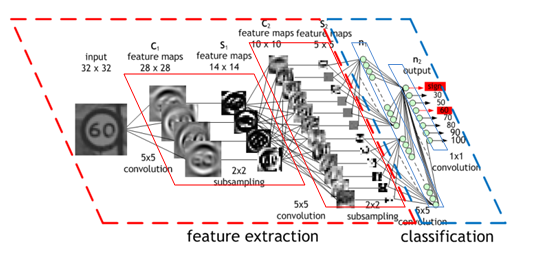
\includegraphics[scale=0.7]{convolutional_neural_network_structure} \]
%   \centering
%   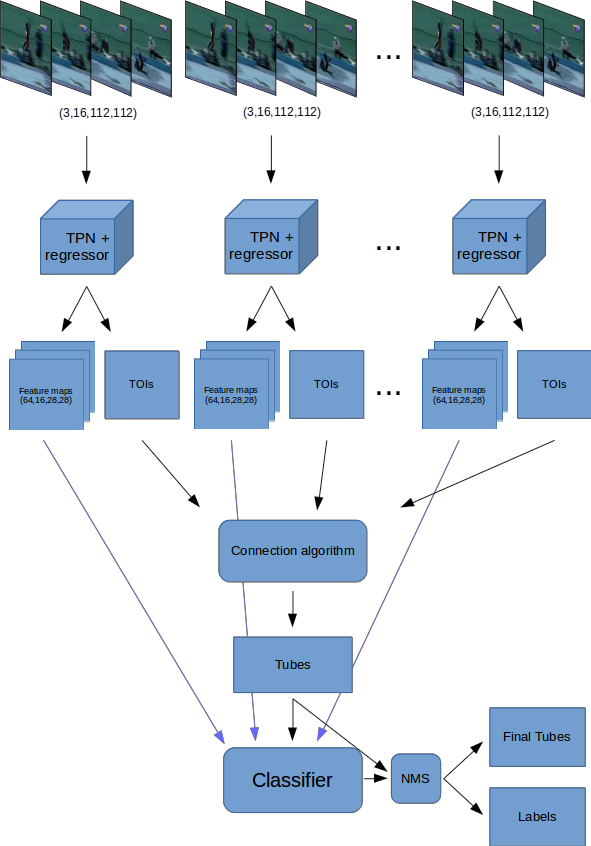
\includegraphics[scale=0.7]{model_nms}
%   \caption{Structure of the network with NMS}
%   \label{fig:network_nms}
% \end{figure}

% \end{document}
